\title{Supplementary Material}
% \section{Practical Relevance}
% \label{postfinance}

% \begin{figure}[!htbp] 
% \centering
% 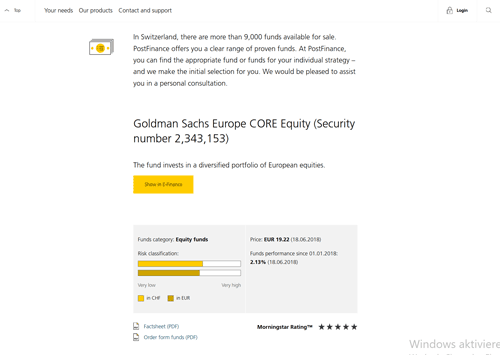
\includegraphics[width=.8\linewidth, keepaspectratio]{Postfinance_Risk_2018Jun19.png} 
% \caption{Information about the risks, that is variance, associated with an investment fund, taken from the consumer webpage of a major Swiss bank (accessed 19. June 2017). The bank explains that "The risk classification is based on the fluctuation range (volatility) of the fund. PostFinance takes the view that risks are very high from a level of 20\% or more. A fund may however be subject to considerably greater fluctuation. The maximum level shown is 20\%"}
% \label{fig:pfrisk}
% %POSTFINANCE:
% % https://www.postfinance.ch/pfch-web/feed-direct/postfinance/vfund/CH0006869207_en.pdf?method=pdf&isin=CH0006869207&lang=en
% % The risk classification is based on the fluctuation range (volatility) of the fund. PostFinance takes the view that risks are very high from a level of 20% or more. A fund may however be subject to considerably greater fluctuation. The maximum level shown is 20%.

% % https://www.postfinance.ch/en/private/products/investing-trading/fund-range.html/feed/fragment/postfinance/fragment2016/funds/fundDetail.jsp?valor=686920&market=393&currency=CHF 
% % retrieved 5.9.2017; 16:58
% \end{figure}

\section{Study 1 -- Supplementary Material}
\subsection{Materials used in Study 1}
\label{sup:study1_material}
\textit{Stimuli.} The material used in Study~1 were the annual returns on investment of stocks of 20 companies. Data about the start and closing values between 2002 and 2015 were obtained, the stocks were the 20 most-traded Swiss stocks at the time of the study (2016), which were: CS Group N,
ABB N,
Swiss Re N,
UBS Group N,
Adecco Group N,
LafargeHolcim N,
Nestle N,
Novartis N,
Swiss Life Hldg N,
Richemont N,
Actelion N,
Syngenta N,
Roche Hldg DR,
Givaudan N,
Geberit N,
The Swatch Grp,
Swisscom Reg,
SGS Reg,
Zurich Insur Grp N,
(Julius Baer Grp N),
SMI.
The stock of Julius Baer was excluded because the available return time series started only 2009. Note that the name of the stocks was not shown to participants. 

\textit{Question wording for variance.} The original question wording (German) of the variance-related questions read as follows: (a, risk) Wie hoch schätzen Sie das Risiko der gezeigten Aktie ein?  (b, variability) Wie hoch schätzen Sie die Variabilität (Varianz) der gezeigten Aktie ein? (c, fluctuation) Wie hoch schätzen Sie die durchschnittliche Schwankung der Rendite der gezeigten Aktie ein? (d, predictability) Wie hoch schätzen Sie die Vorhersagbarkeit der Rendite der gezeigte Aktie ein (gemessen ab 2003)?

\textit{Question wording for gain/loss.} The gain- and loss-related questions read as follows: (a) Wie hoch schätzen Sie den erwarteten durchschnittlichen Verlust (in \%-Punkten) für diese Aktien ein? (b) Wie hoch schätzen Sie den durchschnittlichen Verlust (in \%-Punkten) für die Jahre, in denen die gezeigte Aktie Verluste erzielt hat, ein? (c) Wie hoch schätzen Sie die Wahrscheinlichkeit ein mit der gezeigten Aktie in einem zufällig ausgewähltem Jahr einen Verlust (negative Rendite) zu erzielen? (d) Wie hoch schätzen Sie die durchschnittliche Rendite der gezeigten Aktie ein? (extrem hoher verlust, extrem hoher gewiance Correlations

\subsection{Supplementary Results, Study 1}
\label{study1_supplementary_results}
\subsubsection{Risk-variance Correlation}
\label{study1_risk-variance-correlation}
Correlations between the objective variances and the perceptions of fluctuation, risk, predictability, and variability of the stocks shown in Study~1 (perceived values are z-standardized at the individual level). Simple correlation (pooled across stimuli and participants) between objective variance and perceived fluctuation:
\begin{table}[]
    \centering
    \begin{threeparttable}
    \caption{Study1: Simple correlations between the objective risk (variance) and the perception of stocks}
    \label{sup:tab:study1_rvc}
    \begin{tabular}{lrcrr}\toprule
         & $r$ &  95\% CI & $t$ & $p$ \\
          \midrule
        Perceived fluctuation & $.69$ & $[.67$, $.72]$ & $t(1822) = 41.02$ & $< .001$ \\
        Perceived variation & $.64$ & $[.61$, $.66]$ &  $t(1822) = 35.23$ & $< .001$\\
        Perceived predictability & $-.52$ &  $[-.56$, $-.49]$ & $t(1822) = -26.29$ &  $< .001$\\
        Perceived risk & $.49$ & $[.45$, $.52]$ & $t(1822) = 24.02$ & $< .001$\\
        \bottomrule
    \end{tabular}
    \begin{tablenotes}
    \textit{Note.} Perceived values z-standardized at individual level.
    \end{tablenotes}
    \end{threeparttable}
\end{table}

\begin{table}[H]
\begin{center}
\begin{threeparttable}
\caption{SStudy1: Simple correlations between perceived return and perceived variance
  \label{sup:tab:study1_rrc}}
\begin{tabular}{llrrll}
\toprule
 & \textit{r} & CI1 & CI2 & \textit{t} & \textit{p}\\
\midrule
Fluctuation & 0.11 & 0.07 & 0.16 & 4.75 & 0.00\\
Risk & -0.14 & -0.18 & -0.09 & -5.90 & 0.00\\
Variability & 0.10 & 0.06 & 0.15 & 4.36 & 0.00\\
Predictability & -0.03 & -0.08 & 0.01 & -1.38 & 0.17\\
\bottomrule
\addlinespace
\end{tabular}
\begin{tablenotes}[para]
\normalsize{\textit{Note.} Pearson correlations $r$ from pooled data, subjective values z-standardized at individual level.}
\end{tablenotes}
\end{threeparttable}
\end{center}
\end{table}


For mixed-effects models, it is recommended to report the variance-covariance matrix \cite{Barr2013}. For the model of perceived risk as function of different perceptions of variance, the variance-covariance matrix is shown in Table~\ref{sup:tab:study_1_vcovmat}. 

\begin{table}[H]
\begin{center}
\begin{threeparttable}
\caption{Study1: Variance-covariance matrix of the mixed-effects model with dependent variable perceived return.}
\label{sup:tab:study_1_vcovmat}
\begin{tabular}{llllll}
\toprule
 & \multicolumn{1}{c}{(1)} & \multicolumn{1}{c}{(2)} & \multicolumn{1}{c}{(3)} & \multicolumn{1}{c}{(4)} & \multicolumn{1}{c}{(5)}\\
\midrule
(1) Constant & 0.006 &  &  &  & \\
(2) Perception & 0.000 & 0.000 &  &  & \\
(3) Perception:Risk & 0.000 & 0.000 & 0.001 &  & \\
(4) Perception:Fluctuation & 0.000 & 0.000 & 0.000 & 0.001 & \\
(5) Perception:Variability & 0.000 & 0.000 & 0.000 & 0.000 & 0.001\\
\bottomrule
\addlinespace
\end{tabular}
\begin{tablenotes}[para]
\normalsize{\textit{Note.}  ':' denotes interaction terms. Model specification see footnotes in main text. Predictors were z-standardized at the individual level.}
\end{tablenotes}
\end{threeparttable}
\end{center}
\end{table}

\subsubsection{Study 1: Partial Correlation Details}
Table~\ref{tab:study1_pcc} shows the numerical details of the partial correlation analysis, that is all coefficients and the $p$-values obtained from fitting the partial correlation networks (for implementation details, see main text). Shown are the coefficients for the perceived "risk", "fluctuation", "variability", and "predictability" and the objective risk (variance) and return of the stocks shown during Study~1.

\begin{table}[H]
\begin{center}
\begin{threeparttable}
\caption{\label{tab:study1_pcc}Study 1 results: partial correlations and p-values from the correlation networks.
\label{study1_pcc}}
\begin{tabular}{rccc}
\toprule
 & \multicolumn{1}{c}{Objective Risk (variance)} & \multicolumn{1}{c}{Perceived Return} & \multicolumn{1}{c}{Objective Return}\\
\midrule
\cmidrule{2-4} \textbf{ Perceived Risk } &  &  & \\
\ \ \ Objective Risk (variance) & --- &  & \\
\ \ \ Perceived Return & \textbf{0.09}, $p<.001$ & --- & \\
\ \ \ Objective Return & \textbf{0.38}, $p<.001$ & \textbf{0.3}, $p<.001$ & ---\\
\ \ \ Perceived Risk & \textbf{-0.08}, $ p= 0.00 $ & \textbf{-0.15}, $p<.001$ & \textbf{-0.07}, $ p= 0.00 $\\
\cmidrule{2-4} \textbf{ Perceived Fluctuation } &  &  & \\
\ \ \ Objective Risk (variance) & --- &  & \\
\ \ \ Perceived Return & \textbf{0.1}, $p<.001$ & --- & \\
\ \ \ Objective Return & \textbf{0.39}, $p<.001$ & \textbf{0.32}, $p<.001$ & ---\\
\ \ \ Perceived Fluctuation & -0.04, $ p= 0.08 $ & -0.05, $ p= 0.09 $ & \textbf{0.21}, $p<.001$\\
\cmidrule{2-4} \textbf{ Perceived Variability } &  &  & \\
\ \ \ Objective Risk (variance) & --- &  & \\
\ \ \ Perceived Return & \textbf{0.11}, $p<.001$ & --- & \\
\ \ \ Objective Return & \textbf{0.39}, $p<.001$ & \textbf{0.33}, $p<.001$ & ---\\
\ \ \ Perceived Variability & -0.03, $ p= 0.26 $ & -0.07, $ p= 0.02 $ & \textbf{0.22}, $p<.001$\\
\cmidrule{2-4} \textbf{ Perceived Predictability } &  &  & \\
\ \ \ Objective Risk (variance) & --- &  & \\
\ \ \ Perceived Return & \textbf{0.1}, $p<.001$ & --- & \\
\ \ \ Objective Return & \textbf{0.39}, $p<.001$ & \textbf{0.32}, $p<.001$ & ---\\
\ \ \ Perceived Predictability & \textbf{0.09}, $p<.001$ & 0.04, $ p= 0.19 $ & -0.06, $ p= 0.02 $\\
\bottomrule
\addlinespace
\end{tabular}
\begin{tablenotes}[para]
\normalsize{\textit{Note.} Boldface $=$ significant partial correlations at $\alpha= 0.0125 $}
\end{tablenotes}
\end{threeparttable}
\end{center}
\end{table}

\newpage
\subsubsection{Robustness Check I: Graph Literacy}
Figure~\ref{fig:study1_pcor_by_glit} shows the significant partial correlations after splitting the data at the median graph literacy.
\begin{figure}[H] 
 \centering
 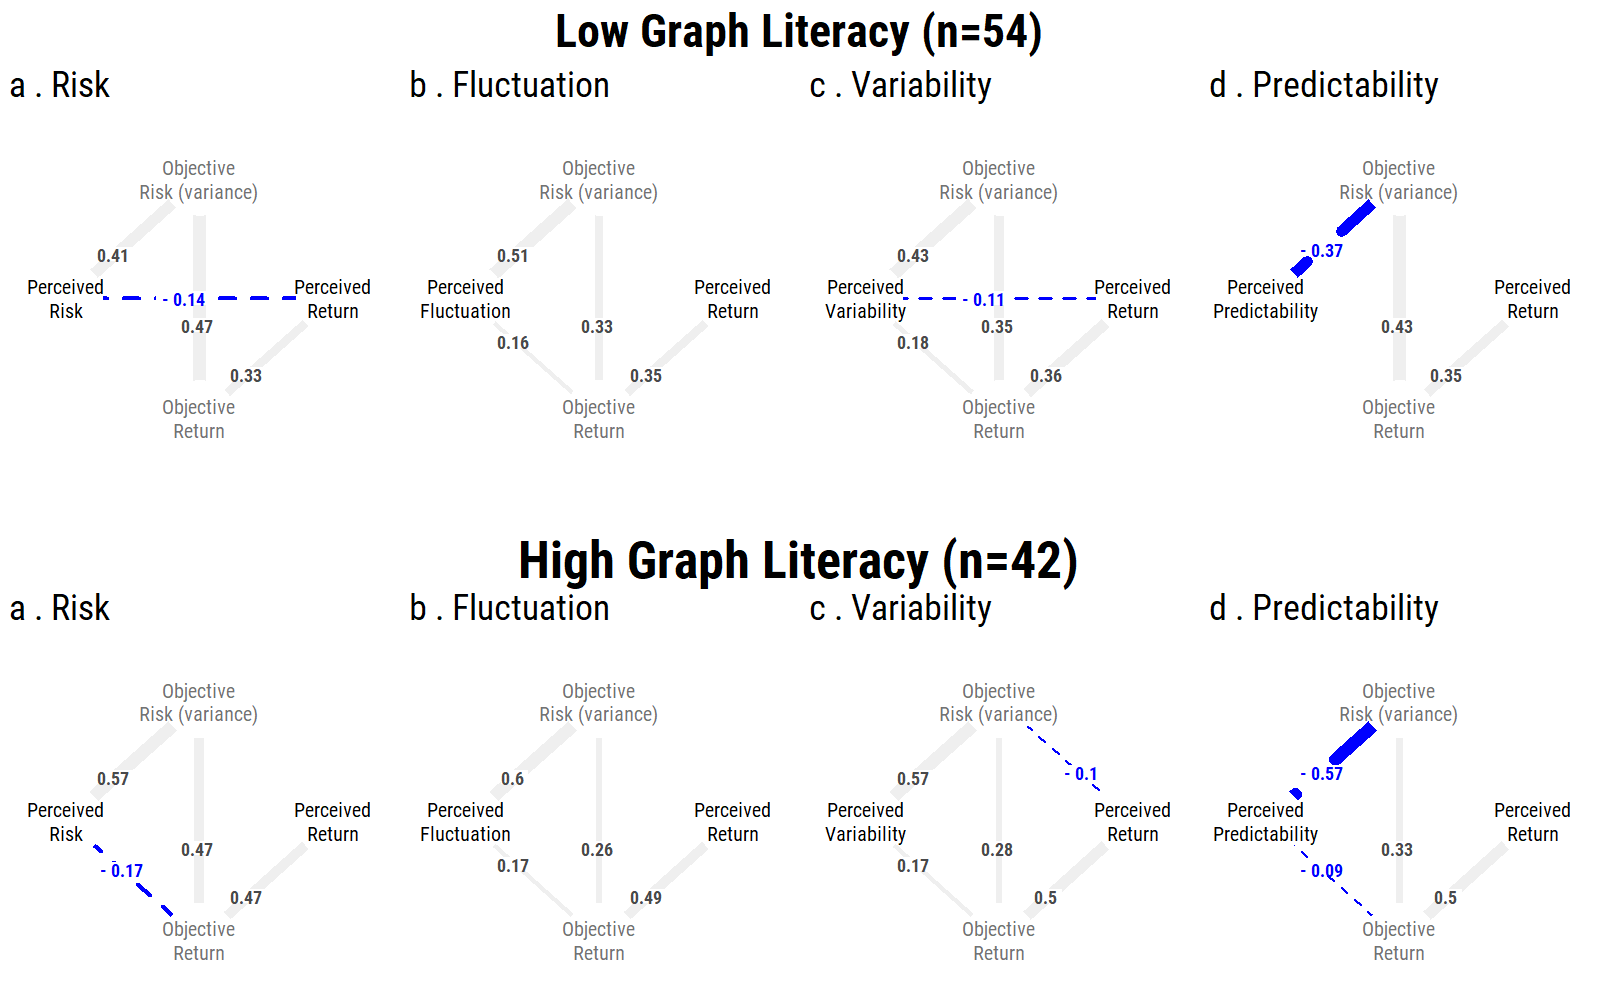
\includegraphics[width=.8\linewidth, keepaspectratio]{sfig1.png} 
 \caption{Partial correlation network, methodology similar to as described int he main text for Study 1, split by graph literacy. Only significant edges are shown, $\alpha=.01$.}
 \label{fig:study1_pcor_by_glit}
\end{figure}

\subsubsection{Robustness Check II: Stock Market Experience}
Figure~\ref{fig:study1_pcor_by_exp}. shows the significant partial correlations after splitting the data into the ones relatively inexperienced with the stock market and the experienced ones.
\begin{figure}[H] 
 \centering
 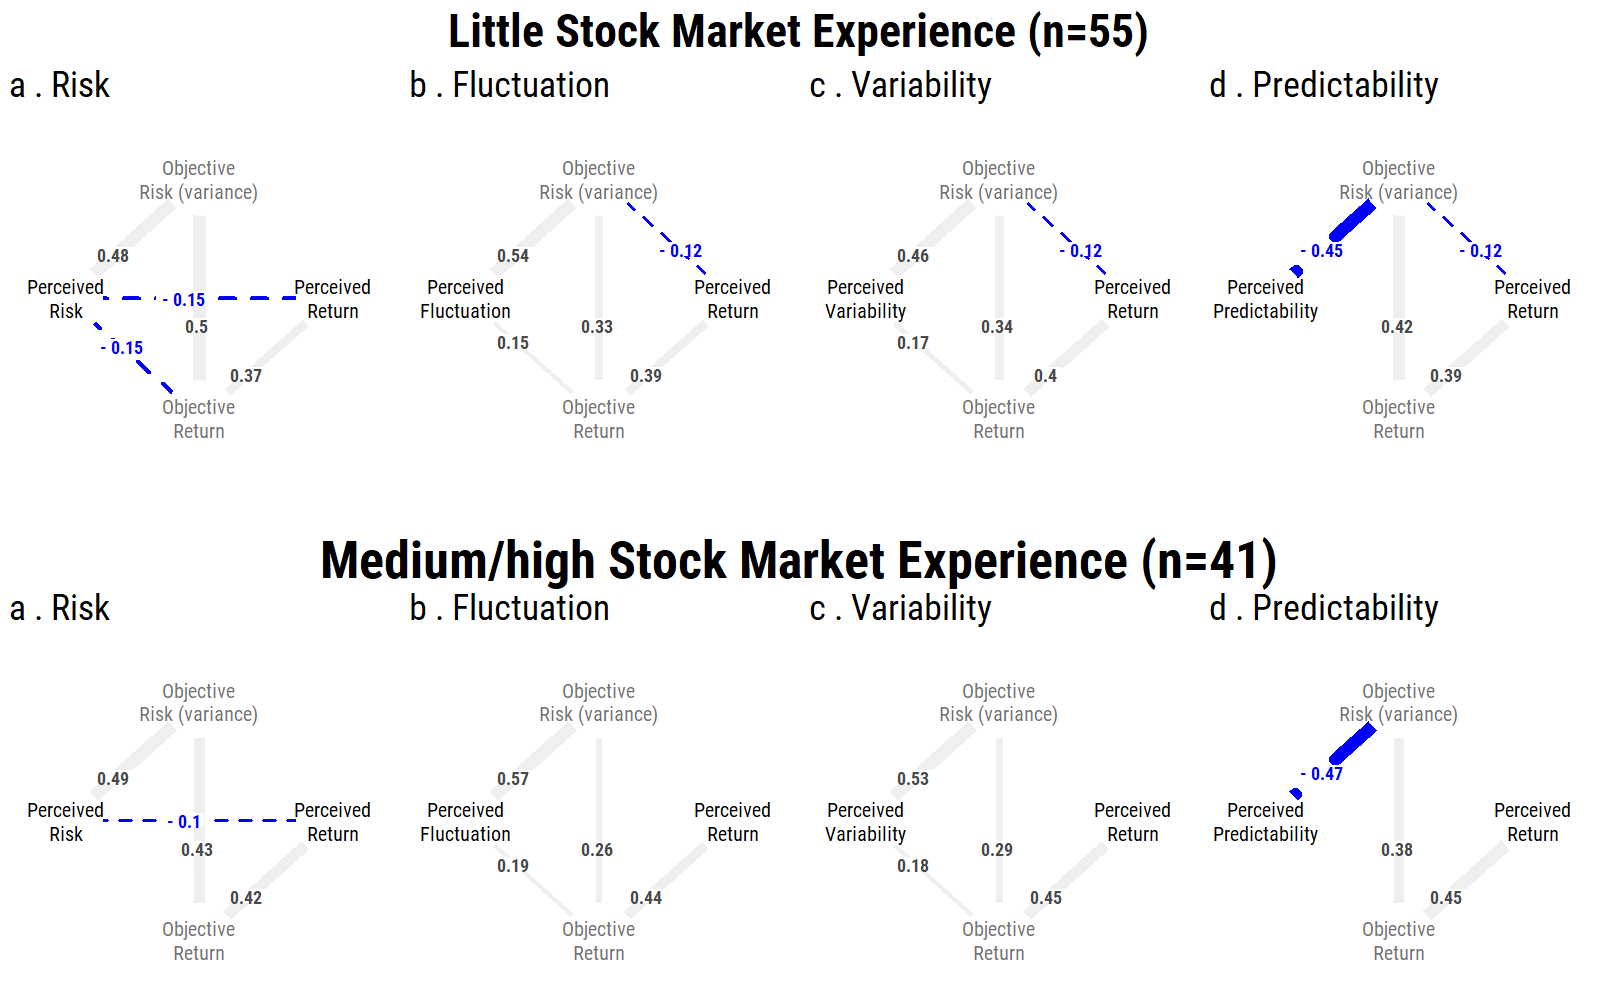
\includegraphics[width=.8\linewidth, keepaspectratio]{sfig2.png} 
 \caption{Partial correlation network, methodology similar to as described in the main text for Study 1, split by experience with the stock market. Only significant edges are shown, $\alpha=.01$.}
 \label{fig:study1_pcor_by_exp}
\end{figure}




%%%%%%%%%%%%%%%%%%%%%%%%%%%%%%%%%%%%%%%%%%%%%%%%%%%%%%%%%%%%%%%%%%%%%%%%%%%%%%%%%%%%%%%%%%





\section{Study 2 -- Supplementary Material}
\subsection{Study 2: Materials}
\label{study2_material}
For Study 2 data from 1 Jan 2009 through 1. Aug. 2017 from price indices of 23 stock markets corresponding to the world's most-traded currencies (as of 2017) were obtained. Only price indices were used. Price indices calculate the value of the index based on the value of the stocks, excluding dividends. Table~\ref{tab:study2_material} lists the indices used in our study. Note: The HSI index (China - Hong Kong, Hang Seng Index) was excluded in favor of the Shanghai Stock Exchange Composite Index (SSE Composite), to avoid that China appears as only country twice in the stimulus material. Also, the German DAX index was excluded in favor of the European EUROSTOXX index, which is also traded in Euro.
% latex table generated in R 3.5.0 by xtable 1.8-3 package
% Fri May 10 15:54:55 2019
\begin{table}[ht]
\centering\small
\caption{Stocks used in study~2} 
\label{tab:study2_material}
\begin{tabularx}{.6\textwidth}{lcc}
  \toprule
Country & Index Fund & ISIN \\ 
  \midrule
Europe & ES50 (EuroStoxx50) & EU0009658145 \\ 
  USA & DJIA & US2605661048 \\ 
  Japan & Nikkei225 & JP9010C00002 \\ 
  United Kingdom & FTSE100 & GB0001383545 \\ 
  Switzerland & SMI20 & CH0009980894 \\ 
  Australia & ASX & XC0009693018 \\ 
  Canada & TSX & XC0009695252 \\ 
  China - Shanghai & SSEC & CNM000000019 \\ 
  Sweden & OMXS30 & SE0000337842 \\ 
  Singapore & FSSTI & XC0009653640 \\ 
  India & BSE & XC0009698199 \\ 
  Russia & RTSI & RU000A0JPEB3 \\ 
  South Africa & JSE (JALSH) & --- \\ 
  Turkey & ISE100 & TRAIMKB00010 \\ 
  Poland & WIG20 & PL9999999987 \\ 
  Argentinia & MERV & ARMERV160025 \\ 
  Indionesia & IDX & --- \\ 
  Malaysia & KLSE & --- \\ 
  Norway & OBX & NO0007035376 \\ 
  Mexiko & MXX & --- \\ 
   \bottomrule
\end{tabularx}
\end{table}



\subsection{Study 2: Supplementary Analyses}
\label{sup:study2_results}
\subsubsection{Correlation Coefficients}
\label{study2_subj_obj_cor}
Table~\ref{tab:study2_subj_obj_cor} shows the correlations between the objective variances of the returns of the index funds and the three perceptions of the variances: risk, fluctuation, and risk (measured as variance), pooled across participants and stimuli. This does not take the clustered nature of the data into account, see below for results controlling for the clustering. The simple correlation is highest for perceptions of fluctuation.
%
\begin{table}[H]
\begin{center}
\begin{threeparttable}
\caption{Study 2: Simple correlations between perceived risk and objective risk (variance)}
\begin{tabular}{lrcrr}
\toprule
  & $r$ & 95\%CI & $t$ & $p$\\
 \midrule
& \multicolumn{4}{c}{With graph}\\
\cmidrule{2-5}
 Perceived risk (measured as variance) & $-.10$ & $[-.16$, $-.03]$ & $t(838) = -2.85$ & $.004$\\
 Perceived risk & $-.19$& $[-.26$, $-.12]$ & $t(798) = -5.54$& $<.001$\\
 Perceived fluctuation & $.19$ & $[.12$, $.25]$ & $t(798) = 5.41$& $<.001$\\
\midrule
 & \multicolumn{4}{c}{Without Graph}\\
 \cmidrule{2-5}
 perceived risk (measured as variance) & $.19$ & $[-.26$, $-.12]$ & $t(778) = -5.47$& $ <.001$\\
 Perceived fluctuation & $-.39$ & $[-.44$, $-.33]$ & $t(798) = -11.81$& $ <.001$\\
 Perceived risk & $-.22$ & $[-.28$, $-.15]$ & $t(818) = -6.33$&  $ <.001$\\
\bottomrule
\addlinespace
\end{tabular}
\begin{tablenotes}[para]
\normalsize{\textit{Note.} $r$: Pearson correlations from pooled data, subjective values z-standardized at individual level.}
\end{tablenotes}
\end{threeparttable}
\end{center}
\end{table}


\subsubsection{Study 2: Objective variance and subjective judgments, pairwise Post-hoc comparisons}
Table~\ref{tab:study2_hlm_trends_pairwise} shows the post-hoc pairwise contrasts between the obtained regression coefficients, regressing objective variance on ratings of risk, fluctuation, and risk (variance), using Tukey p-value adjustments. When graphs are shown, fluctuation perceptions is associatest strongest with the objective variances of the index funds, conpared to risk or risk (variance) perceptions, albeit the effect is small.
% latex table generated in R 3.6.0 by xtable 1.8-4 package
% Mon Jun 17 13:19:48 2019
\begin{table}[H]
\centering
\caption{Pairwise comparisons between trend coefficients, dependent variable: objective risk (variance of the index funds)} 
\label{tab:study2_hlm_trends_pairwise}
\begin{threeparttable}

    
    \begin{tabular}{lrrrrl}
      \toprule
    Contrast & $\Delta$ slope & SE & \textit{df} & $z$-ratio & $p$ \\ 
      \midrule
      & \multicolumn{5}{c}{With Graph}\\
      \cmidrule{2-6}
    risk (variance) - fluctuation & -0.029 & 0.006 & Inf & -4.934 & $<$.0001 \\ 
      risk (variance) - risk & 0.010 & 0.006 & Inf & 1.621 & 0.2366 \\ 
      fluctuation - risk & 0.039 & 0.006 & Inf & 6.477 & $<$.0001 \\ 
       \midrule
       & \multicolumn{5}{c}{Without Graph}\\
       \cmidrule{2-6}
    risk (variance) - fluctuation & -0.014 & 0.006 & Inf & -2.312 & 0.0542 \\ 
      risk (variance) - risk & -0.006 & 0.006 & Inf & -0.991 & 0.5828 \\ 
      fluctuation - risk & 0.008 & 0.006 & Inf & 1.344 & 0.3708 \\ 
       \bottomrule
    \end{tabular}
    \begin{tablenotes}
    \textit{Note.} Slope based on unstandardized effects; p-value adjustment: Tukey for comparing 3 estimates
    \end{tablenotes}
    \end{threeparttable}
\end{table}


% Table created by stargazer v.5.2.2 by Marek Hlavac, Harvard University. E-mail: hlavac at fas.harvard.edu
% Date and time: Mi., Mai 08, 2019 - 16:56:38
\begin{table}[!htbp] \centering \small
 \caption{Study 2: Linear mixed model results. Dependent variable: objective variance of shown stocks} 
 \label{table:supplement_tab1} 
\begin{tabular}{@{\extracolsep{5pt}}lccc} 
\\[-1.8ex]\hline 
\hline \\[-1.8ex] 
 & \multicolumn{3}{c}{Unstandardized b coefficients [range of dep. var. 0.14 $-$ 0.6]} \\ 
\cline{2-4} 
\\[-1.8ex] & (1) & (2) & (3)\\ 
\hline \\[-1.8ex] 
 Graph & $-$0.00 & $-$0.00 & \\ 
 & ($-$.01, .01) & ($-$.01, .01) & \\ 
 & t = $-$0.00 & t = $-$0.00 & \\ 
 & & & \\ \midrule
 Risk x no graph & .04 & & .05 \\ 
 & (.03, .05) & & (.04, .06) \\ 
 & t = 9.59$^{***}$ & & t = 16.89$^{***}$ \\ 
 & & & \\ 
 Risk (variance) x no graph & .03 & & .05 \\ 
 & (.03, .04) & & (.05, .06) \\ 
 & t = 7.93$^{***}$ & & t = 17.79$^{***}$ \\ 
 & & & \\ 
 Fluctuation x no graph & .05 & & .07 \\ 
 & (.04, .06) & & (.07, .08) \\ 
 & t = 11.41$^{***}$ & & t = 24.74$^{***}$ \\ 
 & & & \\ 
 Risk (all) x no graph & & .04 & \\ 
 & & (.04, .04) & \\ 
 & & t = 16.62$^{***}$ & \\ 
 & & & \\ \midrule
 Risk$^{\#}$ x graph & .02 & .08 & \\ 
 & (.01, .03) & (.07, .08) & \\ 
 & t = 3.69$^{***}$ & t = 32.21$^{***}$ & \\ 
 & & & \\ 
 Risk (variance) x graph & .02 & & \\ 
 & ($-$.001, .03) & & \\ 
 & t = 1.89 & & \\ 
 & & & \\ 
 Fluctuation x graph & .03 & & \\ 
 & (.01, .05) & & \\ 
 & t = 3.74$^{***}$ & & \\ 
 & & & \\ \midrule
 Constant & .28 & .28 & .28 \\ 
 & (.28, .29) & (.28, .29) & (.28, .29) \\ 
 & t = 121.40$^{***}$ & t = 120.73$^{***}$ & t = 170.06$^{***}$ \\ 
 & & & \\ 
\hline \\[-1.8ex] 
AIC weight$^{+}$ & 1.00 & 0.00 & 0.00 \\ 
AIC & -7242 & -7197 & -7118 \\ 
BIC & -7177 & -7158 & -7079 \\ 
LogLik & 3631 & 3604 & 3565 \\ 
Random slope & no & no & no \\ 
Random intercept & participant & participant & participant \\ 
\hline 
\hline \\[-1.8ex] 
\textit{Note:} & \multicolumn{3}{l}{$^{*}$p$<$0.05; $^{**}$p$<$0.01; $^{***}$p$<$0.001} \\ 
 & \multicolumn{3}{l}{$^{\#}$For model 2, the predictor 'risk' refers to all question wordings} \\ 
 & \multicolumn{3}{l}{$^{+}$Relative evidence strength, range 0-1 {\citep{Wagenmakers2004}}} \\ 
 & \multicolumn{3}{l}{Predictors are z-transformed.} \\ 
\end{tabular} 
\end{table} 



\subsubsection{Study 2: The risk-return paradox}
Table~\ref{tab:study2_rr} shows the simple correlation coefficients between the perceived return and the perceived risk/risk-as-variance/fluctuation. Note, correlations are pooled (ignoring the repeated measured data structure) and simple (ignoring the inter-correlations between the risk- and return variables in the data).
% latex table generated in R 3.6.0 by xtable 1.8-4 package
% Mon Jun 17 16:02:01 2019
\begin{table}[h!t]
\centering
\caption{Correlation between perceived risk and objective risk (variance)}
\label{tab:study2_rr}
\begin{tabular}{llrr}
 Graph & Question wording & $r$ [95\% CI] & Statistic \\ 
  \midrule
TRUE & risk (variance) & $-.10$, \  $[-.16$, $-.03]$ & $t(838) = -2.85$, $p = .004$ \\ 
   & risk & $-.19$, \  $[-.26$, $-.12]$ & $t(798) = -5.54$, $p < .001$ \\ 
   & fluctuation & $.19$, \  $[.12$, $.25]$ & $t(798) = 5.41$, $p < .001$ \\ 
   \midrule
FALSE & risk (variance) & $-.19$, \  $[-.26$, $-.12]$ & $t(778) = -5.47$, $p < .001$ \\ 
   & fluctuation & $-.39$, \  $[-.44$, $-.33]$ & $t(798) = -11.81$, $p < .001$ \\ 
   & risk & $-.22$, \  $[-.28$, $-.15]$ & $t(818) = -6.33$, $p < .001$ \\ 
   \bottomrule
\multicolumn{4}{l}{{\textit{Note}. Pearson's $r$, pooled data, subjective values z-standardized at individual level.}}
\end{tabular}
\end{table}







\newpage
\subsection{Partial correlation coefficients}
Table~\ref{tab:study2_pcc} shows the numerical details of the partial correlation analysis, i.e. the coefficients and the $p$-values from fitting the partial correlation networks (for implementation details, see main text). Shown are the coefficients for the perceived "risk", "fluctuation", and  "risk (measured as variance)" and return of the index funds that were rated during Study~2.


\begin{sidewaystable}                                                                   

\begin{TableNotes}[para]                                                                                                                                        
\normalsize{\textit{Note.} Significance levels: $^{*} = .05, ^{**} = .01, ^{***} = .001$}                                                                       
\end{TableNotes}                                                                                                                                                
                                                                                                                                                                
\small{                                                                                                                                                         
                                                                                                                                                                
\begin{longtable}{lllllllll}\noalign{\getlongtablewidth\global\LTcapwidth=\longtablewidth}                                                                      
\caption{Study 2 results: partial correlations and p-values from the correlation networks.                                                                      
\label{study1_pcc}}\\                                                                                                                                           
\toprule                                                                                                                                                        
 \multicolumn{4}{c}{With graph} & \multicolumn{4}{c}{Without graph}  &\\                                                                                        
\cmidrule(r){1-4} \cmidrule(r){5-8}                                                                                                                             
 & \multicolumn{1}{c}{1} & \multicolumn{1}{c}{2} & \multicolumn{1}{c}{3} & \multicolumn{1}{c}{4} & \multicolumn{1}{c}{1} & \multicolumn{1}{c}{2} & \multicolumn{1}{c}{3} & \multicolumn{1}{c}{4}\\                                                                                                                              
\midrule                                                                                                                                                        
\endfirsthead                                                                                                                                                   
\caption*{\normalfont{Table \ref{tab:} continued}}\\                                                                                                            
\toprule                                                                                                                                                        
 \multicolumn{4}{c}{With graph} & \multicolumn{4}{c}{Without graph}  &\\                                                                                        
\cmidrule(r){1-4} \cmidrule(r){5-8}                                                                                                                             
 & \multicolumn{1}{c}{1} & \multicolumn{1}{c}{2} & \multicolumn{1}{c}{3} & \multicolumn{1}{c}{4} & \multicolumn{1}{c}{1} & \multicolumn{1}{c}{2} & \multicolumn{1}{c}{3} & \multicolumn{1}{c}{4}\\                                                                                                                              
\midrule                                                                                                                                                        
\endhead                                                                                                                                                        
Risk &  &  &  &  &  &  &  & \\                                                                                                                                  
\ \ \ 1 Perceived Risk &  &  &  &  &  &  &  & \\                                                                                                                
\ \ \ 2 Perceived Return & $-0.20^{**}$ &  &  &  & $-0.14$ &  &  & \\                                                                                           
\ \ \ 3 Objective Risk (variance) & $\hphantom{-}0.44^{***}$ & $-0.01$ &  &  & $\hphantom{-}0.13^{***}$ & $\hphantom{-}0.02$ &  & \\                            
\ \ \ 4 Objective Return & $-0.13^{**}$ & $\hphantom{-}0.32^{***}$ & $\hphantom{-}0.55^{***}$ &  & $\hphantom{-}0.02$ & $-0.02$ & $\hphantom{-}0.58^{***}$ & \\ 
\ \ \ 5 Positive Attitude & $-0.09^{*}$ & $\hphantom{-}0.16^{***}$ & $\hphantom{-}0.03$ & $-0.21^{***}$ & $-0.17^{***}$ & $\hphantom{-}0.27^{***}$ & $-0.01$ & $-0.11^{**}$\\                                                                                                                                                   
Risk-as-variance &  &  &  &  &  &  &  & \\                                                                                                                      
\ \ \ 1 Perceived Risk-as-variance &  &  &  &  &  &  &  & \\                                                                                                    
\ \ \ 2 Perceived Return & $-0.19^{**}$ &  &  &  & $-0.11$ &  &  & \\                                                                                           
\ \ \ 3 Objective Risk (variance) & $\hphantom{-}0.51^{***}$ & $\hphantom{-}0.05$ &  &  & $\hphantom{-}0.13^{**}$ & $\hphantom{-}0.00$ &  & \\                  
\ \ \ 4 Objective Return & $-0.10^{*}$ & $\hphantom{-}0.38^{***}$ & $\hphantom{-}0.53^{***}$ &  & $\hphantom{-}0.08^{*}$ & $-0.05$ & $\hphantom{-}0.57^{***}$ & 
\\                                                                                                                                                              
\ \ \ 5 Positive Attitude & $-0.13^{**}$ & $\hphantom{-}0.13^{**}$ & $-0.03$ & $-0.13^{***}$ & $-0.11^{*}$ & $\hphantom{-}0.29^{***}$ & $-0.01$ & $-0.08^{*}$\\ 
Fluctuation &  &  &  &  &  &  &  & \\                                                                                                                           
\ \ \ 1 Perceived Fluctuation &  &  &  &  &  &  &  & \\                                                                                                         
\ \ \ 2 Perceived Return & $\hphantom{-}0.07$ &  &  &  & $-0.22^{***}$ &  &  & \\                                                                               
\ \ \ 3 Objective Risk (variance) & $\hphantom{-}0.65^{***}$ & $-0.10^{*}$ &  &  & $\hphantom{-}0.17^{***}$ & $-0.02$ &  & \\                                   
\ \ \ 4 Objective Return & $\hphantom{-}0.04$ & $\hphantom{-}0.37^{***}$ & $\hphantom{-}0.38^{***}$ &  & $\hphantom{-}0.05$ & $-0.08$ & $\hphantom{-}0.56^{***}$ & \\                                                                                                                                                           
\ \ \ 5 Positive Attitude & $-0.09^{*}$ & $\hphantom{-}0.06$ & $\hphantom{-}0.05$ & $-0.15^{***}$ & $-0.15^{**}$ & $\hphantom{-}0.29^{***}$ & $-0.03$ & $-0.09^{*}$\\                                                                                                                                                           
\bottomrule                                                                                                                                                     
\addlinespace                                                                                                                                                   
\insertTableNotes                                                                                                                                               
\end{longtable}                                                                                                                                                 
                                                                                                                                                                
}

\end{sidewaystable}






\subsubsection{Linear model comparison for perceived return}
Data-driven selection of the (hierarchical) linear model that we used in the main text based on complexity-penalized goodness of fit (AIC). Dependent variable was perceived return, the fixed effects were question$\times$perceived variance, graph$\times$perceived variance, objective variance, objective return. Predictors question and graph were effects coded. The random effects structure is varied, see the different rows in the table, where row 1 contains a fixed-effects only model and the last row the maximum random effects structure of interest. For all models, variance inflation factors ($VIF$) were at maximum 2 ($VIF > 5$ indicates problematic multicollinearity).
% latex table generated in R 3.6.0 by xtable 1.8-4 package
% Fri Jun 21 08:49:47 2019
\begin{table}[H]
\centering
\caption{Study 2: Linear model comparison, dependent variable: perceived return} 
\label{tab:study2_lm_return_modelcomparison}
\begin{tabular}{p{4.3cm}cccccccr}
  \toprule
 & Df & AIC & BIC & logLik & deviance & $\chi^2$ & $\chi^2$Df & Pr(>$\chi^2$) \\ 
  \midrule
Fixed effects only & 10 & 14791 & 14855 & -7385 & 14771 &  &  &  \\ 
  Interc. by id & 11 & 14504 & 14575 & -7241 & 14482 & 289 & 1 & 0.000 \\ 
  Interc. by index & 11 & 14612 & 14683 & -7295 & 14590 & 0 & 0 & 1.000 \\ 
  Interc. \& slope by id & 13 & 13517 & 13601 & -6745 & 13491 & 1099 & 2 & 0.000 \\ 
  Interc. \& slope by index & 13 & 14611 & 14695 & -7293 & 14585 & 0 & 0 & 1.000 \\ 
  Interc. \& slope by id + Interc. \& slope by index & 16 & 13308 & 13412 & -6638 & 13276 & 1309 & 3 & 0.000 \\ 
   \bottomrule
   \multicolumn{9}{l}{\small\textit{Note}. Variables were centered at the Likert scale midpoints.}\end{tabular}
\end{table}


\begin{table}[H]
\begin{center}
\begin{threeparttable}
\caption{Study 2 results: Mixed-effects model, estimated slopes for the predictor attitude. Dependent variable: perceived return}
\label{sup:tab:study2_attitude_lm_trends}
\begin{tabular}{lccrrr}
\toprule
Question & Slope & SE & df & \textit{z}-ratio & \textit{p}\\
\midrule
& \multicolumn{5}{c}{No Graph}\\
\cmidrule{2-6}
Risk & 0.344 & 0.044 & \$\textbackslash{}infty\$ & 7.819 & 0.000\\
Risk (measured as variance) & 0.358 & 0.043 & \$\textbackslash{}infty\$ & 8.323 & 0.000\\
Fluctuation & 0.448 & 0.047 & \$\textbackslash{}infty\$ & 9.511 & 0.000\\
\midrule
& \multicolumn{5}{c}{Graph}\\
\cmidrule{2-6}
Risk & 0.145 & 0.041 & \$\textbackslash{}infty\$ & 3.501 & 0.000\\
Risk (measured as variance) & 0.085 & 0.041 & \$\textbackslash{}infty\$ & 2.087 & 0.037\\
Fluctuation & 0.077 & 0.038 & \$\textbackslash{}infty\$ & 2.058 & 0.040\\
\bottomrule
\end{tabular}
\begin{tablenotes} \small
    \textit{Note.} Model specification as in Footnote 12 of the main text, but adding to the frixed effects the attitude score as main effect ans as interaction term.
\end{tablenotes}
\end{threeparttable}
\end{center}
\end{table}
